\label{sec:evaluation}

All evaluations listed in this section are running 
on a quiescent Intel Core 2 dual-processor system with 16GB RAM. In this machine, each processor is consisted of 4-core 64-bit Intel Xeon, running at 2.33 GHz with a 4MB shared L2 cache and 32KB private L1 cache. The underlying operating system is unmodified CentOS 5.5 with Linux 2.6.18-194.17.1.el5. The \texttt{glibc} version is 2.5.

In order to compare performance fairly, all benchmarks were built as 64-bit executables using LLVM compiler (clang-3.2) with optimization ``-O2''. 

This section is going to answer the following questions:
\begin{itemize}
\item
How is the performance overhead of \doubletake{} ~\ref{sec:perf}?

\item
How is the memory overhead of \doubletake{}~\ref{sec:memoverhead}?

\item
How effective is \doubletake{} on detecting heap buffer overflows, memory leakage and memory usage-after-free errors~\ref{sec:effect}? 


\end{itemize}

\subsection{Performance Overhead}
\label{sec:perf}

\begin{figure*}[ht]
\begin{center}
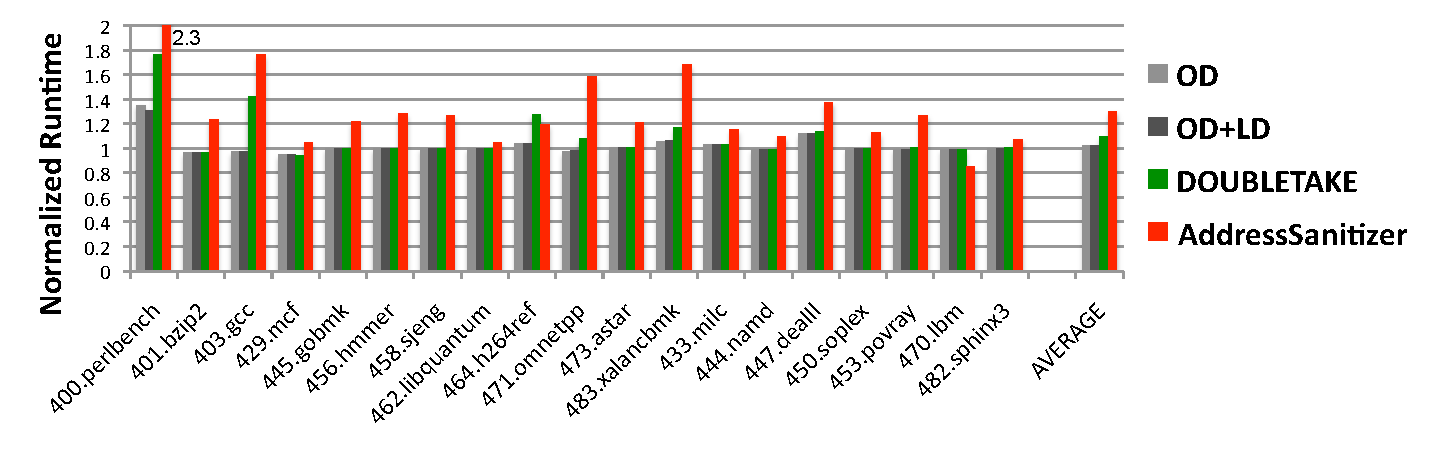
\includegraphics[width=6.5in]{figure/perf}
\end{center}
\caption{
Performance overhead of \doubletake{} and AddressSanitizer.
\label{fig:perf}}
\end{figure*}

We evaluate performance on all C/C++ benchmarks in SPEC CPU2006, totally 19 benchmarks. We compare \doubletake{} with AddressSanitizer and Valgrind. AddressSanitizer is the state-of-the-art tool of detecting buffer overflow and usage-after-free memory errors ~\cite{AddressSanitizer}, but cannot detect memory leakage. Valgrind is a widely used tool to detect memory leakage and other memory errors ~\cite{overflow:valgrind}. 

we disable the rollback and re-execution mechanism for \doubletake{} in order to show the performance overhead of normal execution, the common path for a program without memory errors. For a fair comparison, we disable the instrumentation on reads and the checking for the stack and the globals for AddressSanitizer. We run every benchmark three times and show the average performance for \doubletake{} and AddressSanitizer. The variance on the observed performance for these three different execution is under 1\% and not listed here.   
Because Valgrind is running more than $10\times$ slower, we only evaluate Valgrind once. Also, we kill a program if it is already running $20\times$ slower, including 400.perlbench, 458.sjeng, and . Thus, the performance of Valgrind is worse than the data showed here. 

Performance are showed in Figure~\ref{fig:perf}. Averagely, \doubletake{} only introduces 9\% performance overhead for detecting heap overflows, memory leakage and memory use-after-free errors. To compare, AddressSanitizer performance overhead is about 30\% and Valrind is more than \textbf{10 $\times$}). For 17 out of 19 test cases, \doubletake{} performs better than AddressSanitizer, even with an additional functionality to check memory leakage. For 12 test cases, \doubletake{}'s performance overhead is omittable, less than 3\%. \doubletake{} substantially outperforms Valrind for all of these evaluated benchmarks. 

From the figure, we also observe that \doubletake{} introduces more than 7\% performance overhead for six benchmarks, including 400.perlbench, 403.gcc, 464.h264ref, 471.omnetpp, 483.xalancbmk, and 447.dealII. We further evaluate the overhead caused by different applications on these benchmarks. Results are showed in Figure ~\ref{fig:perfdetails}. From this figure, we observe that most overhead is coming from the component of detecting memory use-after-free errors. As described in Section~\ref{sec:danglingpointer}, \doubletake{} has to fill the first 128 bytes with canaries. If an application has a big number of memory allocation and de-allocation, filling canaries consists of the most significant overhead. When we remove the detection of memory use-after-free errors, performance overhead are dropping down from 9\% to less than 3\%, which are not shown here because of page limit. 

\begin{figure}
\begin{center}
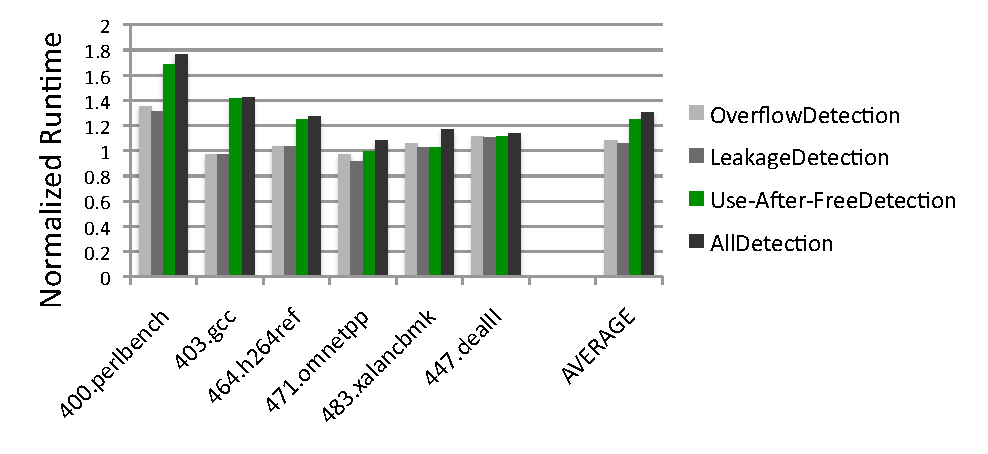
\includegraphics[width=3.4in]{figure/perfdetails}
\end{center}
\caption{
\doubletake{} performance overhead for different applications.
\label{fig:perfdetails}}
\end{figure}

\label{sec:memoverhead}


\subsection{Memory Overhead}
\begin{figure*}
\begin{center}
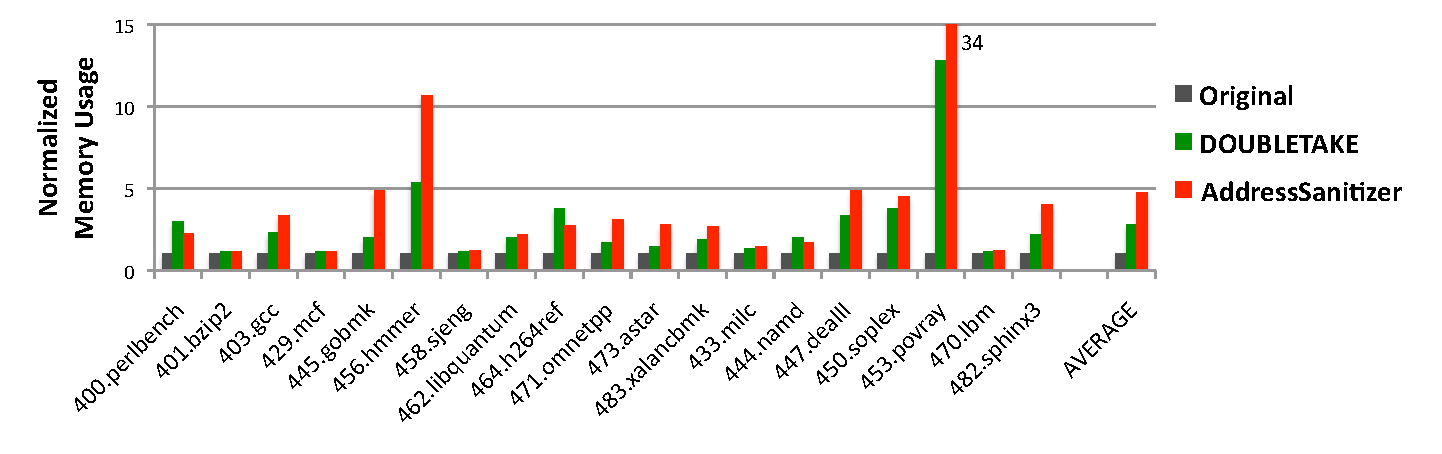
\includegraphics[width=6.5in]{figure/memory}
\end{center}
\caption{
Memory overhead of \doubletake{} and AddressSanitizer.
\label{fig:memory}}
\end{figure*}

\label{sec:memoverhead}
Memory overhead of \doubletake{} comes from the following aspects. Firstly, snapshot in the beginning of each epoch, by backing up the globals, the heap and the stack, contributes the most significant memory overhead of \doubletake{}. However, if there is only one epoch in an application, \doubletake{} does not introduce too much memory overhead for the snapshot. That explains less than $2\times$ memory overhead in seven benchmarks. Secondly, recording results of system calls introduce some memory overhead. Also, different applications may introduce different memory overhead. For the detection of heap buffer overflows and memory leakage, \doubletake{} adds canaries around each heap object and maintains a bit map to indicate canary locations. For the detection of memory usage-after-free errors, \doubletake{} delays memory re-usage by putting freed objects into a quarantine list, which also introduces constant additional memory overhead. 

We evaluate the physical memory overhead here because \doubletake{} pre-allocates a huge block of heap, which is 4GB virtual memory and should not be counted as memory overhead. Proportional set size (PSS) in \texttt{/proc/self/smaps} reflects physical memory increase on the existing system by running an application. Thus, we periodically collect this data and use the sum of different memory mappings as total physical memory usage. We presents the maximum value of  running different benchmarks in Figure~\ref{fig:memory}. 

Averagely, \doubletake{}'s memory overhead is 2.8$\times$, while AddressSanitizer's overhead is 4.8$\times$. For all benchmarks except perlbench and namd, \doubletake{} has lower memory overhead. It is worth noting that the total memory usage for all benchmarks of \doubletake{} is less than 2$\times$ of original memory usage. 
 
\subsection{Effectiveness}
\label{sec:effect}

\subsubsection{Micro Benchmarks}
{\bf Heap Overflows}: We evaluate \doubletake{} on 26 test cases from NIST SAMATE Reference Dataset Project, see Table~\ref{table:SAMATESRDOverflow}. \doubletake{} can detect all buffer overflows when they corrupted canaries and does not have any false alarms. Test cases 1955 and 2063 are not detected by \doubletake{} because they are not continuous buffer overflows, which cannot be detected by any canary-based approaches.

{\bf Memory Leakage}: We evaluate 13 test cases listed in Table~\ref{table:SAMATESRDLeak}. \doubletake{} reports memory leakage correctly for all test cases.  

{\bf Memory Usage-After-Free}: 
{Use After Free}
  
\begin{comment}
SAMATE Reference Dataset Project. http://samate.nist.gov/SRD/.TEST cases from National Institute of Standards and
Technology. SAMATE Reference Dataset Project. http://samate.nist.gov/SRD/.

\begin{table}[!t]
\centering
\begin{tabular}{l|r}
\hline
{\bf \small Vunerbility Class} & {\bf \small SRD Test Case ID} \\
\hline
strcpy & 015 \\
strcpy & 1843 \\
strcpy & 1845 \\ % Array Index 
memory opration & 1952 \\ % Memory operation
Array Boundary & 1955 \\ % Array assignment
Array Boundary & 1958 \\ % Array assignment
Array Index & 1961 \\ % Array assignment
Array Index & 2062 \\ % Array assignment
Array Index & 2063 \\ % Array assignment
Array Index & 2064 \\ % Array assignment
Array Index & 2065 \\ % Array assignment
Array Index & 2145 \\ % Array assignment
strcpy & 2147 \\ % Array assignment

\hline \\ 
% Good Cases
strncpy & 1844 \\
strcpy & 1846 \\ % Array Index, limit string 
strcpy & 1848 \\
strcpy & 1936 \\
Memory & 1953 \\
Array Boundary & 1956 \\ % Array assignment
Array Boundary & 1959 \\ % Array assignment
Array Index & 1962 \\ % Array assignment
Array Index & 2066 \\ % Array assignment
Array Scope & 2067 \\ % Array assignment
Array Index & 2068 \\ % Array assignment
strcpy & 2134 \\ % Array assignment
strcpy & 2148 \\ % Array assignment
strcpy & 2149 \\ % Array assignment
 
\hline
\end{tabular}
\caption{SAMATE Test Cases. 
\label{table:SAMATESRD}}
\end{table}
\end{comment}


\begin{table}[!t]
\centering
\begin{tabular}{l|l}
\hline
{\bf \small Vulnerable Cases } & {\bf \small Good Cases} \\
\hline
015 1843 1845 1952 1955 & 1844 1846 1848 1936 1953\\
1958 1961 2062 2063 2065 & 1956 1959 1962 2066 2067 \\
2145 2147 & 2068 2134 2148 2149\\  
\hline
\end{tabular}
\caption{SAMATE Test Cases for Heap Overflows. 
\label{table:SAMATESRDOverflow}}
\end{table}

\begin{table}[!t]
\centering
\begin{tabular}{l|l}
\hline
{\bf \small Memory Leakage } & {\bf \small Good Cases} \\
\hline
1527 1583 1758 1925 1926 & 1458 1584 1587\\
1933 2056 99201 99202 99203 &   \\
\hline
\end{tabular}
\caption{SAMATE Test Cases for Memory Leakage. 
\label{table:SAMATESRDLeak}}
\end{table}


\subsubsection{Real Applications}

\begin{table}[!t]
\centering
\begin{tabular}{l|l|l}
\hline
{\bf \small Buffer Overflows} & {\bf \small Memory Leakage} & {\bf \small Use-after-free}\\
\hline
bc libhx & & \\
\hline
\end{tabular}
\caption{Evaluated Real Applications. 
\label{table:realapps}}
\end{table}

For buffer overflows, we have evaluate the effectiveness on  . Most of them have been included in
bugbench~\cite{}. 

For memory leakage problem, since we already found a lots of memory leakage in \texttt{perlbench}
and \texttt{gcc} benchmarks of SPEC2006, we evaluate real \texttt{perl} and \texttt{gcc} applications, {\bf PERL-... } and {\bf GCC-***} using the same input used in SPEC2006. 
Those memory leakage are still in these newest applications. 

For memory usage-after-free problems, 
In this section, we eveluate that 
LBC evaluate its effectiveness on bugbench.
bc, man and polymorph have overflow bugs.
gzip, ncompress exploit overflows using strcpy. 

%% RIPE: benchmark
%% Nullhttpd: two bound violations. We can't evaulate this problem because it is multithreaded program. 
%SAMATE:  

%Also, some from the Cruiser,
wu-ftpd, sudo, cvs, libhx, lynx
bc: two heap overflow
To check the effectiveness on the real applications, \doubletake{} evaluated all test cases listed in Table~\ref{}. They all coming from previous works. 


urrently, we have evaluated libhx successfully.

